\chapter{绪论}

\section{引言}
子痫前期(preeclampsia, PE)又作先兆子痫,是孕妇妊娠期特有的一种多系统进展性疾病, 与妊娠期高血压(gestational hypertension)、子痫(eclampsia)、
慢性高血压并发子痫前期(chronic hypertension with superimposed preeclampsia)以及妊娠合并慢性高血压(chronic hypertension)统称妊娠期
高血压疾病(hypertension disorders of pregnancy, HDP)\cite{OAG9,HDASOM,2000s1}。
子痫前期临床表现的显著特点是原发性高血压与蛋白尿。
近年来,组织的对子痫前期的涵盖范围进行了进一步的拓展,在妊娠20周后出现新发(原发)高血压,在两次间隔$4h$或$4h$以上的血压测定中,收缩压≥$140mmHg$和(或)
舒张压≥$90mmHg$,且伴有下列任一项或多项\cite{OAG9,FIGO}:

一、蛋白尿

孕妇出现蛋白尿症状,尿蛋白≥$300mg/24h$,或尿蛋白/肌酸酐比值≥$30mg/mol$,或随机尿蛋白≥(+)。

二、器官受损

孕妇无尿蛋白但伴有以下任一器官或系统功能紊乱、受累受损:心、肺(肺水肿)、肝(血清转氨酶水平为正常值2倍以上)、肾(血肌酐水平大于$1.1mg/dl$
或为正常值2倍以上)等重要器官,或血液系统(血小板<$100 \times 10^{9}/L$)等)、消化系统、神经系统的异常改变等。

三、胎盘-胎儿受到累及

胎盘胎儿生长受限、脐动脉多普勒分析检测异常、死胎等。

妊娠期高血压疾病可引起严重的母胎并发症,是孕产妇和围产儿病死率升高的主要原因\cite{OAG9}。
据世界卫生组织统计,子痫前期在孕妇中发病率高达5\%-10\%,是除体内大出血外孕妇死亡的第二大危险因素\cite{LCT2006},每年可导致全球范围内约76 000名孕妇死亡,并进一步导致约500 000
名胎儿/婴儿的死亡\cite{DAM2015,LCT2006}(如\autoref{fig:dhd}所示)。为推广普及人们对危及母婴生命安全的子痫前期的认知,同时教育女性了解她们当前及长期的健康风险,
全球孕妇保健组织自2017年起将每年的5月22日确定为世界子痫日(world preeclampsia day)(如\autoref{fig:wpd}所示)。
\begin{figure}[htbp]
    \centering
    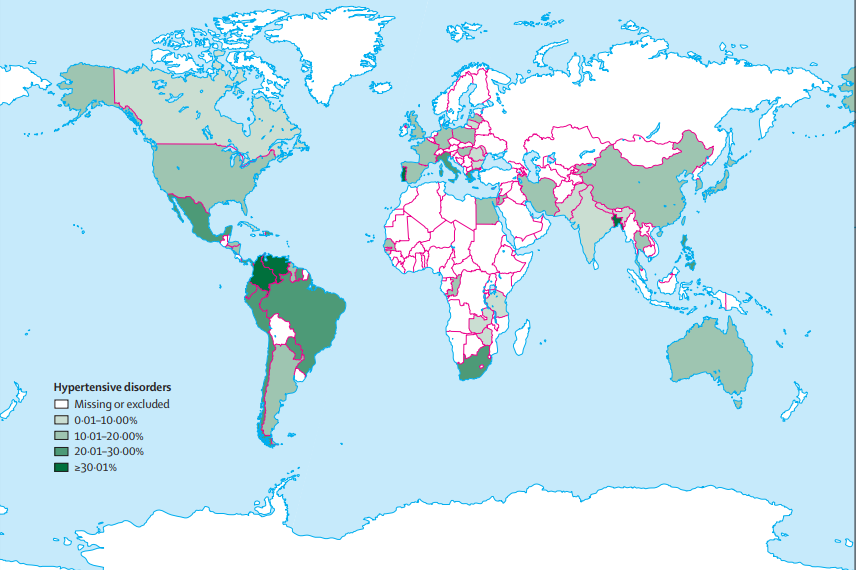
\includegraphics[width=.5\linewidth]{ch1/dhd}
    \caption{\label{fig:dhd}因妊娠期高血压疾病死亡孕妇的国家分布比例}
\end{figure}
\begin{figure}[htbp]
    \centering
    
\includegraphics[width=.5\linewidth]{ch1/wpd}
    \caption{\label{fig:wpd}2021年世界子痫日主题:Preeclampsia: Beyond Pregnancy}
\end{figure}

就现阶段我国国情而言,由于人口基数大、人口出生率较高,导致每年妊娠孕妇数及新生儿数总量大。
同时,自全面开放二孩政策后,各地区高龄孕妇、二次妊娠孕妇比例明显提升。而临床研究已经证实,
高龄与二(三)次妊娠均属于可能导致子痫前期的风险因素,会增加孕妇子痫前期的患病可能。

因此,如何对子痫前期快速有效的医学诊断与干预成为新的难题,实现子痫前期的预测和及早诊断,
是对孕妇子痫前期的治疗及孕妇、围生儿的健康安全的保障,具有重大的临床应用价值。
\section{子痫前期的病理及危害}
\subsection{病因及发病机制}
截止目前,医学界对子痫前期的病因与发病机制尚未完全明确,相关研究还在继续进行之中。但得到公认的一点是,子痫前期病发具有异质性,多因素、多机制及多通路均对子痫前期的发病有所影响,不能仅以“一元论”的观点对待。
目前临床对子痫前期的病因和发病机制的主要有以下几种学说:

一、子宫螺旋小动脉重铸不足

该学说认为子痫前期的发病与妊娠早期胎盘功能紊乱密切相关\cite{OAG9,Duvekot2010},其作用机制可以概括为两个阶段,如\autoref{fig:ppp}所示。
在第一阶段,孕妇子宫螺旋动脉重构受损、出现重铸障碍,绒毛外滋养细胞浸润能力受损,导致胎盘缺血、缺氧,释放多种胎盘因子,该阶段无明显临床现象;在第二阶段,各种胎盘因子进入母体血液循环,血管阻力增大,胎盘灌注减少,
促进系统性炎症反应的激活及血管内皮损伤引起子痫前期-子痫多样化的临床表现。尽管造成子宫螺旋小动脉重铸足的机制尚待研究,该学说是目前临床最为普遍接受的。
\begin{figure}[htbp]
    \centering
    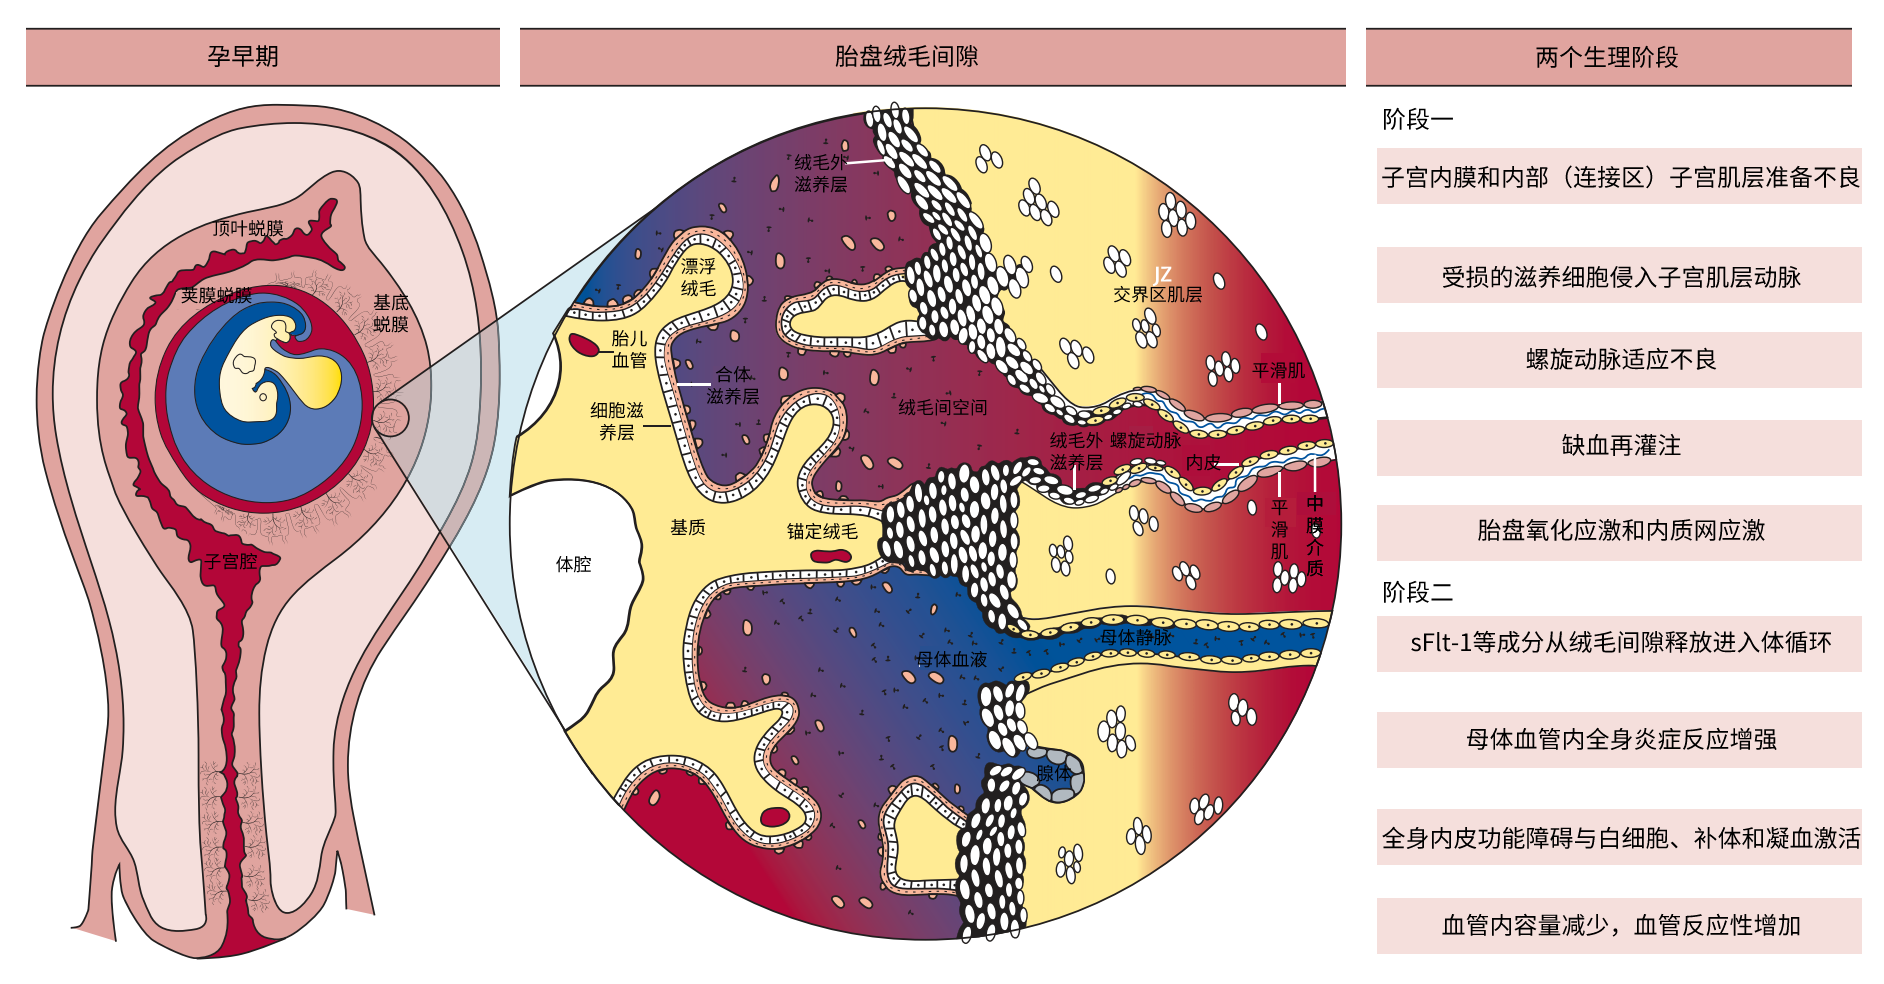
\includegraphics[width=.7\linewidth]{ch1/ppp}
    \caption{\label{fig:ppp}一种子痫前期可能的发病机制}
\end{figure}

二、炎症免疫过度激活

该学说认为子痫前期是母系-父系免疫适应不良导致的\cite{Sibai2005,OAG9,Shi2006},即胎儿胎盘具有的半抗原性移植体特性导致同种异体移植排斥,最终引起的母系同种免疫反应从而诱发子痫前期。
精子内有组织相容性的白细胞分化抗原(HLA)存在,很多学者已发现当母体滋养细胞不能够表达足够强的移植物抗原(HLA-A, HLA-B, HLA-D)\cite{Moffett2002}时,母体T细胞是无法识别HLA的,
从而使母体对胚胎免疫耐受降低。妊高征患者HLA抗体的检出率明显高于正常孕妇、妊高征患者体液免疫与细胞免疫功能异常等临床现象都能与免疫学说较好的验证。

三、血管内皮细胞损伤及前列腺素合成失调

该观点认为,当血管内皮细胞出现损伤后,将进一步导致前列腺素合成失调\cite{OAG9,Sibai2005}。它使扩血管物质如一氧化氮(NO)、前列环素(PGI2),合成减少,而缩血管物质如内皮素(ET)、血栓索(TXA2)等合成增加,从而促进血管痉挛。
此外血管内皮损伤还可使抗凝血酶(ATⅢ)减少并激活血小板及凝血因子进入母体血循环,导致凝血功能增加,纤溶活性抑制,加之血管痉挛,内皮细胞损伤,胶原暴露,激发血管内凝血,甚至是血栓的出现。

四、遗传因素

子痫前期具有家族倾向性,提示遗传因素与该病发生有关\cite{OAG9,Sibai2005}。临床研究发现子痫前期主要体现为母系遗传,家系分析发现\cite{Ge2013},妊高征患者一级亲
属及二级亲属的发病率比无家族史孕妇明显增高,这表明孕妇对妊高征有遗传易患性,且目前多倾向于多基因遗传,其具体的遗传规律目前尚有争议。由于子痫前期的异质性,尤其是遗传
和环境因素的交互作用产生了复杂的表型。在子痫前期遗传易感性研究中,尽管目前已定位了十几个子痛前期染色体易感区域,但在该区域内进一步寻找易感基因仍面临很大的挑战。

五、其他学说

近几年来,学者们还相继提出一些新的可能引起子痫前期的学术观点,如胎盘因子学说\cite{Shi2006}等。同时一些临床研究也发现,多种营养因素如低白蛋白血症、钙、镁、锌、硒等缺乏与子痫前期发生发展
可能有关\cite{OAG9}。但此类学说与假设仍需进一步临床研究与理论研究来证实。

\subsection{子痫前期引起的生理变化及危害}
子痫前期引起的基本的病理生理变化是全身小动脉痉挛、血管内皮损伤和水钠潴留。全身各脏器各系统灌注减少,对母儿造成危害,甚至导致母儿死亡。由于该病表现为多脏器和系统损害,故有学者提出子痫前期
-子痫综合征(preeclampsia-eclampsia syndrome)的概念。

一、全身小动脉痉挛 

可能由于升压系统和降压系统平衡失调,血管壁对某些升压物质(如血管紧张素Ⅱ)的反应性增强,从而使全身小动脉,特别是直径200um以下的小动脉发生痉挛,导致各器官供血不足,外周阻力增高,产生高血压等一系列症状体征。

子宫血管痉挛,胎盘供血不足,绒毛退行性变、出血、坏死、梗塞等,导致胎盘提高老化,功能不全。病变进行缓慢时,可致胎儿宫内生长发育迟缓(IUGR),病变急剧时,可致胎死宫内,严重时胎盘后小血管破裂,导致胎盘早剥。

脑部血管痉挛,脑组织缺氧、水肿、严重时出血,出现头昏、头痛、恶心、呕吐,重者抽搐、昏迷,脑疝形成而致死亡。

心脏血管痉挛,心肌缺血、间质水肿、点状出血及坏死,加之血液粘稠度增加,外周阻力增加,心脏负担加重,可导致左心衰竭,继而发生肺水肿。

肾脏血管痉挛,肾血流量减少,组织缺氧,血管壁通透性增加,血浆从肾小球漏出,出现蛋白尿及管型。肾小球毛细血管痉挛,肾小球内皮细胞肿胀,发生血管内凝血,纤维蛋白沉着,肾小球滤过率减少,出现尿少,严重者出现肾功衰竭。

肝脏由于缺血,肝细胞线粒体内所含的谷丙转氨酶释放,可致血清谷丙转氨酶升高,出现黄疸表明病情严重。肝脏主要病变为门静脉周围有局限性出血,继而纤维素性血栓形成,严重者肝实质缺血坏死、肝包膜下出血。

眼底小动脉痉挛、缺血、水肿,严重时渗出、出血,甚至视网膜剥离,出现眼花、视物模糊,甚至失明。

二、水钠潴留 

可能由于肾小球滤过率减少,肾小管对钠的重吸收增加,钠离子潴留细胞外而引起水肿。肾上腺皮质激素、抗利尿激素分泌增加,也可能是水潴留的另一个原因。由于水钠潴留,组织水肿,体重异常增加。

\section{子痫前期的研究现状}
现代医学对子痫前期的认知经历了漫长的探索\cite{BJOG2016},如\autoref{fig:history}所示。早在古希腊希波克拉底(Hippocrates)时代(约公元前460-370年),医学界就对子痫的症状有一定的认识。但直至18世纪,医学界才将子痫与癫痫加以区分对待。
19世纪中叶,医学界开始认识到子痫之前存在一个前驱状态。此外,法国医生Pierre Rayer首次描述了子痫孕妇的蛋白尿症状,英国医生John Lever更进一步证实了蛋白尿与子痫发病的特异性关系。
20世纪初,尿液分析与血压测量开始用于子痫的诊断,同时,进一步细化的子痫前期的相关概念开始出现。20世纪中后叶,由于医学诊断技术的发展,多种新的检测指标与技术不断被引入子痫及子痫前期的识别诊断中。
进入21世纪后,由于智能化设备的发展,基于医学大数据的人工智能相关研究又成为了新的热点。
\begin{figure}[htbp]
    \centering
    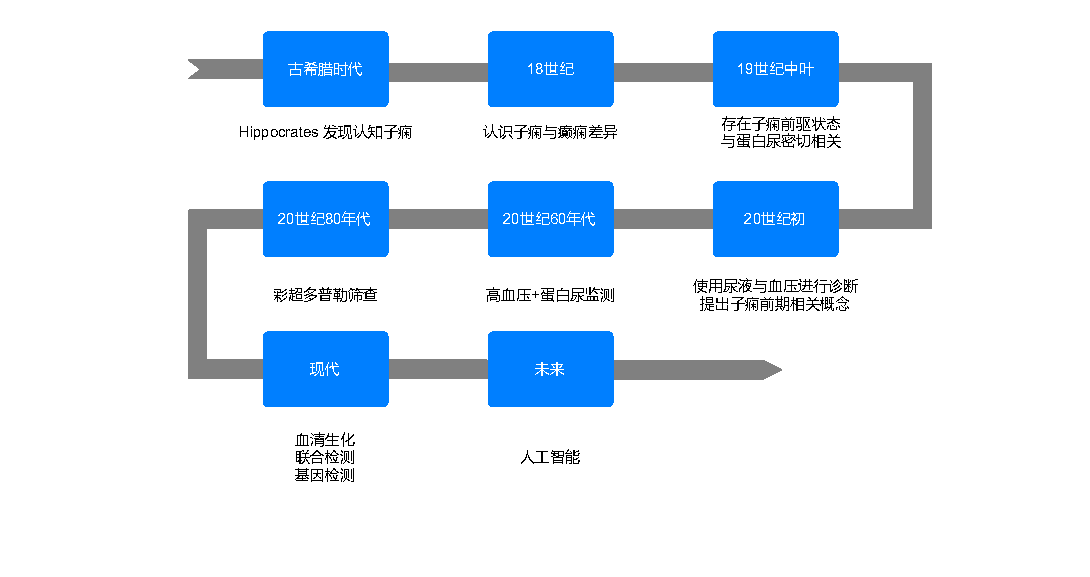
\includegraphics[width=.8\linewidth]{ch1/history}
    \caption{\label{fig:history}医学界对子痫及子痫前期研究简史}
\end{figure}

本小节将从现阶段临床对子痫前期发生评估的常用参数、临床检测设备及新兴人工智能检测技术等三方面对子痫前期进行介绍。
\subsection{检测参数}
一、风险因子

已有研究表明,许多孕妇自身风险因子与子痫前期的发生密切相关\cite{Magee2008,FIGO,Lowe2015,Heazell2010}。临床医生往往会以量表问卷的形式向孕妇采集这些信息,
对孕妇罹患子痫前期的可能进行初筛\cite{risks},如\autoref{fig:risk}所示。常见的子痫前期风险因子包含以下几点:
\begin{figure}[htbp]
    \centering
    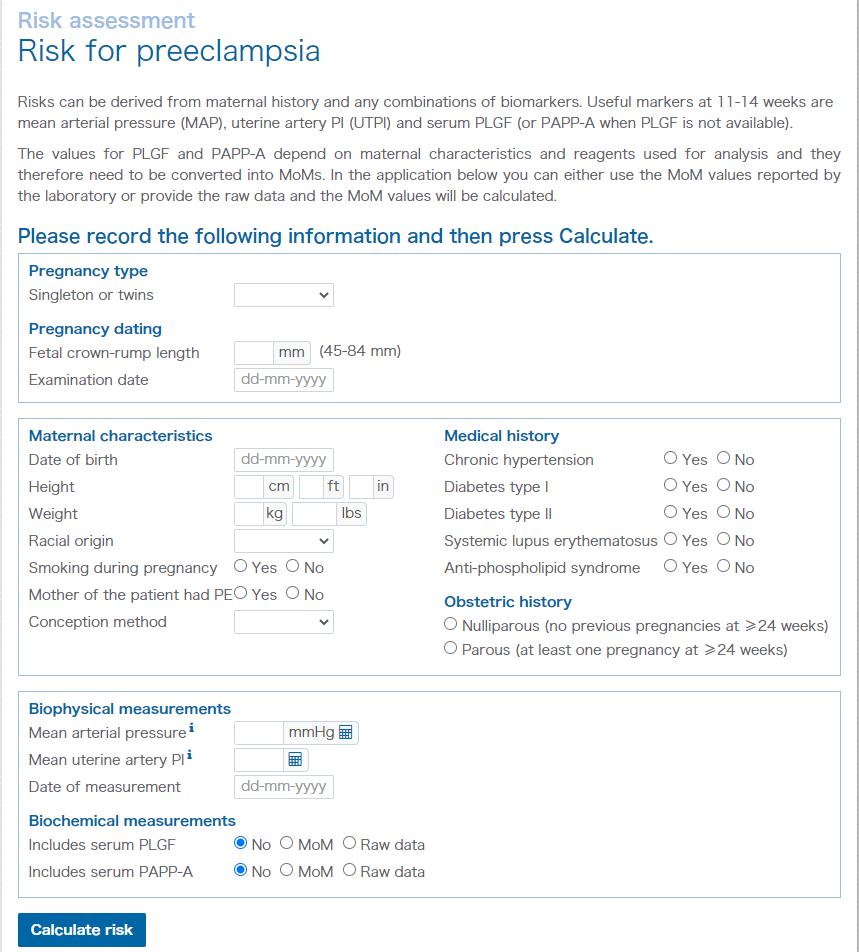
\includegraphics[width=.6\linewidth]{ch1/risk}
    \caption{\label{fig:risk}子痫前期风险因子评估量表}
\end{figure}

1. 产妇年龄

有证据显示,高龄孕妇(分娩时年龄超过35周岁)发生子痫前期的可能将增加1.2-3倍;当孕妇年龄大于35周岁时,其发生子痫可能增加;当年龄超过40周岁时,其发生子痫前期的可能将
增加两倍\cite{Duckitt2005,FIGO,Yogev2010}。
多项研究评估了子痫前期与孕妇年龄的风险,多元回归分析统计显示,当孕妇年龄超过32周岁时,孕妇年龄每增加1年,其发生子痫的可能增加4\%;当孕妇年龄超过34岁时,这一数值将激增至30\%。
但孕妇的年龄与其增加发生原发子痫前期的可能无关,即使年轻的孕妇仍有可能发生子痫前期\cite{Duckitt2005,Poon2010}。

2. 胎产次

临床统计发现,初产孕妇患子痫前期的可能会增加。多项人口统计显示,这一感染风险甚至能达到惊人的三倍以上\cite{Lee2000,Duckitt2005,Coonrod1995}。另外一项调查研究显示,
没有既往子痫前期病史的经产孕妇患子痫前期可能的风险会降低\cite{Robillard1993}。

3. 既往史

2009年,Sonia等人对1987年至2004年间的763 795名首次分娩的产妇的相关数据进行了分析统计,结果显示首次分娩产妇罹患子痫前期的概率比未患有子痫前期既往史的二胎孕妇风险更大\cite{Sonia2009}。
对已分娩的妇女而言,在以后的妊娠中发生子痫前期的风险则与既往子痫前期发病史有很大关联,二次妊娠中发生子痫前期的相对风险可提高7-10倍\cite{Duckitt2005,CAMPBELL1985,Lie1998,Sibai1986}。

4. 妊娠间隔

临床研究证实,多次妊娠间隔时间过长或过短都会在一定程度上增加PE发生的风险\cite{Rousso2002,Duckitt2005,Conde2007}。2016年,Mignini等人\cite{Mignini2016}对拉丁美洲1990年-2009年间的894 479名孕妇进行了统计
分析,结果显示与孕妇二次妊娠间隔12-23个月相比,妊娠间隔不到12个月或超过72个月则会增加PE患病风险。Rolv\cite{Rolv2002}等人对挪威的551 478名多次妊娠孕妇的研究调查显示PE既往史对孕妇二次妊娠具有短暂
的保护作用,孕妇二次妊娠的PE患病风险与上次分娩后经过的时间直接相关。

5. 辅助生殖

多项临床研究显示,当孕妇通过辅助生殖技术(assisted reproductive technologies,ART)受孕时,其PE患病可能会增加一倍\cite{Jackson2004,Trogstad2009}。 Angela S. Martin等人\cite{Martin2016}的研究显示,
不论通过何种具体ART受孕的孕妇与自然受孕的孕妇相比,其患子痫前期的风险均有所增加。这一结果可能ART过程中雌激素水平过高可能导致胎盘受损和子宫胎盘循环减少以及子宫螺旋动脉血管浸润的减少有关。

6. 家族史

临床研究统计显示,PE在一定程度上显现出家族性易感性\cite{ARNGRIMSSON1990,OAG9,Williams2011}。(曾)患有PE的女性的女儿或姐妹发展成PE的可能性是没有家族PE史的女性的3-4倍\cite{ARNGRIMSSON1990,Cincotta1998,FIGO,Williams2011}。但PE具体遗传方式与机制尚不明确。

7. 肥胖

多项临床统计表明,若孕妇出现肥胖症状($BMI>30kg/m^2$),则其PE患病可能会增加2-4倍\cite{Williams2011,FIGO,Zintzaras2006}。但肥胖与PE的具体作用机制尚不清楚。另一方面,由于出现肥胖的孕妇往往是高龄孕妇,其患慢性高血压的可能也较大。但排除掉这些因素可能的影响,
肥胖仍然会导致PE患病风险增加\cite{Duckitt2005}。另一方面,Sebire等人\cite{Sebire2001}在2001年的一项研究表明,当孕妇BMI指数<20时,其PE风险显著降低,则从侧面验证了肥胖对PE的影响。

8. 种族

人口统计研究表明,不同民族、区域、肤色的孕妇其子痫患病可能会有一定的差异\cite{Ghosh2014,Khalil2013}。

9. 并发症

当孕妇自身已患有某些疾病或感染某些症状时,其PE患病可能也会增加\cite{FIGO,Ray2016,OAG9}。临床研究已证实,这些疾病包括胰岛素依赖型糖尿病\cite{Lee2000,Garner1990}、肾病\cite{Martinell1990}、
慢性自身免疫病\cite{Stamilio2000}及抗磷脂综合症\cite{Dreyfus2001,Marchetti2016}等。

二、生理生化指标筛查

筛查PE的另一种方法是基于贝叶斯定理,将单个孕妇的PE风险因子和及其母体特征病史的先验风险与其进行的各项生物物理、生物化学检测结果相结合,从而估计其PE患病风险\cite{FIGO}。这一过程即为参数估计中的极大后验概率估计
(maximum a posterori,MAP),即按照观测值判断当前值x最可能属于哪一类进行分类决策\cite{Qiu2012}。不失一般性,以二元检测问题为例,MAP分类过程可以表示为
\begin{equation}
    \label{equ:maxap}
    H_{x}=
    \left \{
    \begin{aligned}
        &H_{1}, \text P(H_{1}|x)&>P(H_{0}|x), \\
        &H_{1}, \text P(H_{1}|x)&<P(H_{0}|x),
    \end{aligned}
    \right.  
\end{equation}
其中,$P(H|x)$为观测值x属于$H$的后验概率,选出从观测值x所有类别中选出后验概率最大的,即为观测值所属类别。上述筛选过程9中孕妇的生理、生化检测结果统称为生物标志物(biomarker),生理参数主要包括血压、子宫动脉搏动指数等,生化参数
(biomarker)则种类繁多、新参数层出不穷\cite{Rene2008,Zhong2015,Zeisler2016,Rana2012},这里选取血清妊娠相关蛋白A(Pregnancy associated plasma protein A,PAPP-A)与血清胎盘成长因子(placental growth factor,PLGF)为代表进行介绍。

1. 血压

由于PE是妊娠期高血压疾病的一种\cite{OAG9,HDASOM,2000s1},血压对PE的影响和意义不言而喻。血压值一直以来是临床用以对PE监测、诊断的重要指标。测量血压时,孕妇同一手臂应至少测量两次,收缩压>140mmhg和或舒张压>90mmhg定义为高血压。
对首次发现血压身高的孕妇,应至少间隔4小时后再次测量确认\cite{OAG9}。除基本的收缩压(systolic blood pressure,SBP)、
舒张压(diastolic blood pressure,DBP)外,平均动脉压(mean arterial pressure,MAP)更是作为国际妇产科联盟的建议指标,用于实际标定诊断PE之中,其计算方法如\autoref{equ:map}所示\cite{FIGO}。
\begin{equation}
    \label{equ:map}
    MAP=DBP+(SBP-DBP)/3
\end{equation}
Leona C.Y. Poon\cite{Poon2008}等人对5590名单胎孕妇的一项研究表明,当单独使用MAP进行检测时,PE的检测率为38\%;当结合孕妇病史等因素时,PE检出率可达63\%,假阳性率为10\%。
Stamilio等人\cite{Stamilio2000}发现,孕妇第一次产前检查时出现MAP>90毫米汞柱与其PE患病的可能相关性显著。

2. 子宫动脉搏动指数

UTPI是国际妇产科联盟与妇产科超声学会所推荐的对PE进行筛查的参数之一\cite{FIGO,Sotiriadis2019}。\autoref{fig:utpi}展示了一例孕早期经腹多普勒超声检查子宫动脉的结果\cite{Sotiriadis2019}。
UTPI本质上也是一种血液动力学参数,其基本定义与MAP类似,是子宫动脉收缩期峰值流量$A$减去舒张末期流量$B$除以平均流量$M$\cite{Cnossen2008}:
\begin{equation}
    \label{equ:utpi}
    UTPI=\frac{A-B}{M}
\end{equation}
同时,常与UTPI一起检测的还有子宫动阻力动指数(Resistance index,RI)、子宫动脉(peak systolic to late diastolic ratio,S/D R)及切迹等参数\cite{Cnossen2008}。
\begin{figure}[htbp]
    \centering
    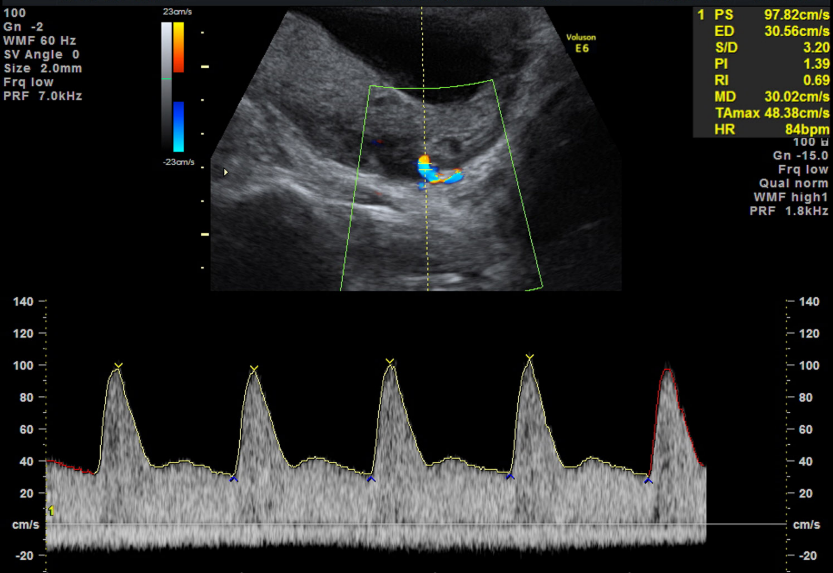
\includegraphics[width=.6\linewidth]{ch1/utpi}
    \caption{\label{fig:utpi}孕早期经腹多普勒超声检查子宫动脉}
\end{figure}
Jeltsje S. Cnossen等人\cite{Cnossen2008}此前众多学者研究的回顾表明,在孕妇妊娠$11^{+0}-13^{+6}$周时,若子宫动脉多普勒血流检测发现UTPI上升或出现子宫动脉舒张早期切迹等印象,则该孕妇PE患病的可能将增加\cite{OAG9,Plasencia2008}。

3.血清妊娠相关蛋白A

PAPP-A是由细胞滋养层分泌的一种金属蛋白胰岛素生长因子结合蛋白,在胎盘的生长发育中起着重要的作用。PE已被证明与低水平的PAPP-A循环有关\cite{FIGO}。但相关临床研究表明,仅使用PAPP-A单指标无法准确预测PE\cite{Smith2002}。
因此,PAPP-A常与其他检测参数一起配合使用\cite{Poon2009,Tan2018,Ray2018}。 

4. 胎盘生长因子

PLGF是由绒毛状细胞滋养层膜细胞滋养层合成,是一种糖基化二聚糖蛋白,具有血管生成合血管修复的功能。临床研究显示,PLGF的血管生成功能在妊娠过程中会发挥很大作用,PLGF水平或其抑制受体水平的变化可能与PE的发生有关\cite{Levine2004,Ahmad2004}。
同时,临床证据表明,在孕早期患有PE的孕妇其PLGF的浓度较正常妊娠孕妇更低\cite{Chau2017}。
2019年,Duhig等人\cite{Duhig2019}对1019名疑似PE的孕妇进行了追踪实验,在整个实验期间一直持续性的进行PLGF水平检测。结果显示,针对实验组(n=573),PE诊断时间的中位数为4.1天,而对照组(n=446)这一数值仅为1.9天,证明PLGF可以有效的缩短PE确诊的时间。
2015年,Zhong等人\cite{Zhong2015}对多项血清生化指标在PE预测方面的性能进行了比较,结果显示,PLGF的综合性能优于其他诸如胎盘蛋白13(Plancenta protein 13,PP13)、PAPP-A
等其他血清生化指标。鉴于此,\textbf{FIGO组织特别将胎盘生长因子推荐为PE检测首选生化指标}\cite{FIGO}。

\subsection{分析及检测设备}
一、标准医疗设备

目前临床所使用的PE筛查检测设备主要以检测生化标志物为主,国内外医疗器械公司研发推出了一系列软硬件综合分析系统。但整体而言,国内医疗器械设备公司研发起步晚,检测指标较国外设备数目少。

1. 德国勃拉姆斯公司的产前检测设备

勃拉姆斯公司(B·R·A·H·M·S GmbH)一直致力于对各种生物标志物检测的研究中,其公司产品KRYPTOR GOLD与KRYPTOR compact PLUS\cite{B·R·A·H·M·S2021}可完成对AFP、Free $\beta$hCG、$\beta$hCG、PAPP-A、PlGF、
sFlt-1、uE3等在内的多种生物标志物的检测,
满足PE的早期筛查及诊断等多种应用场景,如\autoref{fig:B·R·A·H·M·S}所示。同时该公司还研发了一套Fast Screen pre I plus$^\text{TM}$综合软件分析系统,可结合检测结果对孕妇PE发病可能进行风险评估。

\begin{figure}[htbp]
    \centering
    \subfigure[KRYPTOR GOLD]{
    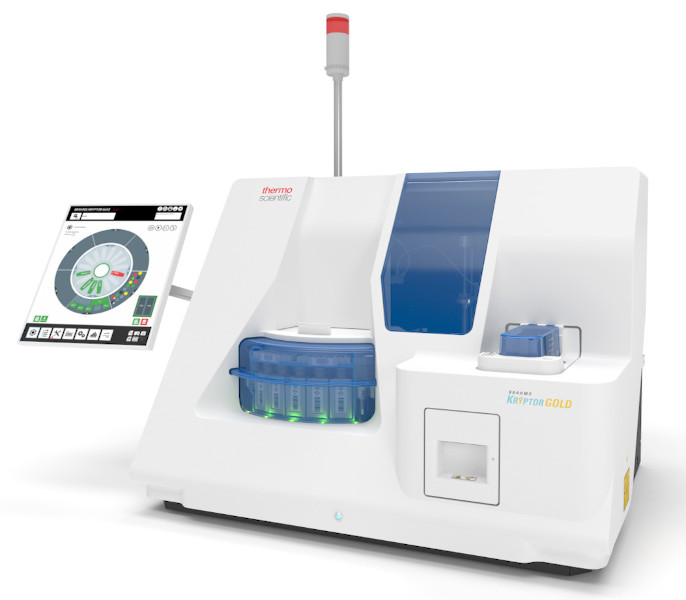
\includegraphics[width=5.5cm]{ch1/brahms-kryptor-gold-686}
    }
    \quad
    \subfigure[KRYPTOR compact PLUS]{
    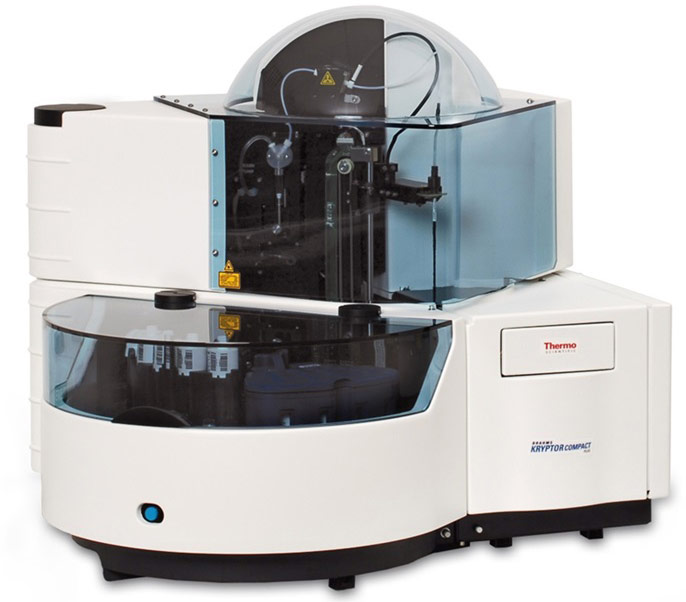
\includegraphics[width=5.5cm]{ch1/brahms-kryptor-compact-plus-686}
    }
    \caption{\label{fig:B·R·A·H·M·S}勃拉姆斯公司KRYPTOR系列的两款检测设备}
\end{figure}
2.美国珀金埃尔默公司的产前检测设备

珀金埃尔默公司(PerkinElmer)提供全面的筛查和诊断解决方案组合,推进早期临床检测在成医疗领域的应用。该公司针对PE在内的多种孕期综合并发症提出了完整的检测方案,其AutoDELFIA系列、
VICTOR2系列及DELFIA Xpress系列的多款免疫荧光分析仪平台\cite{perkinelmer2021}均可完成对AFP、Free $\beta$hCG、$\beta$hCG、PAPP-A、PlGF、
sFlt-1、uE3等在内的PE生物标志物检测标定,如\autoref{fig:PerkinElmer}所示。此外,该公司位硬件检测设备配套研发了LifeCycle软件分析系统,实现了从样品接收-检验检测-风险评估-化验报告的全自动工作流程。
\begin{figure}[h]
    \centering
    \subfigure[VICTOR2 D荧光检测仪]{
    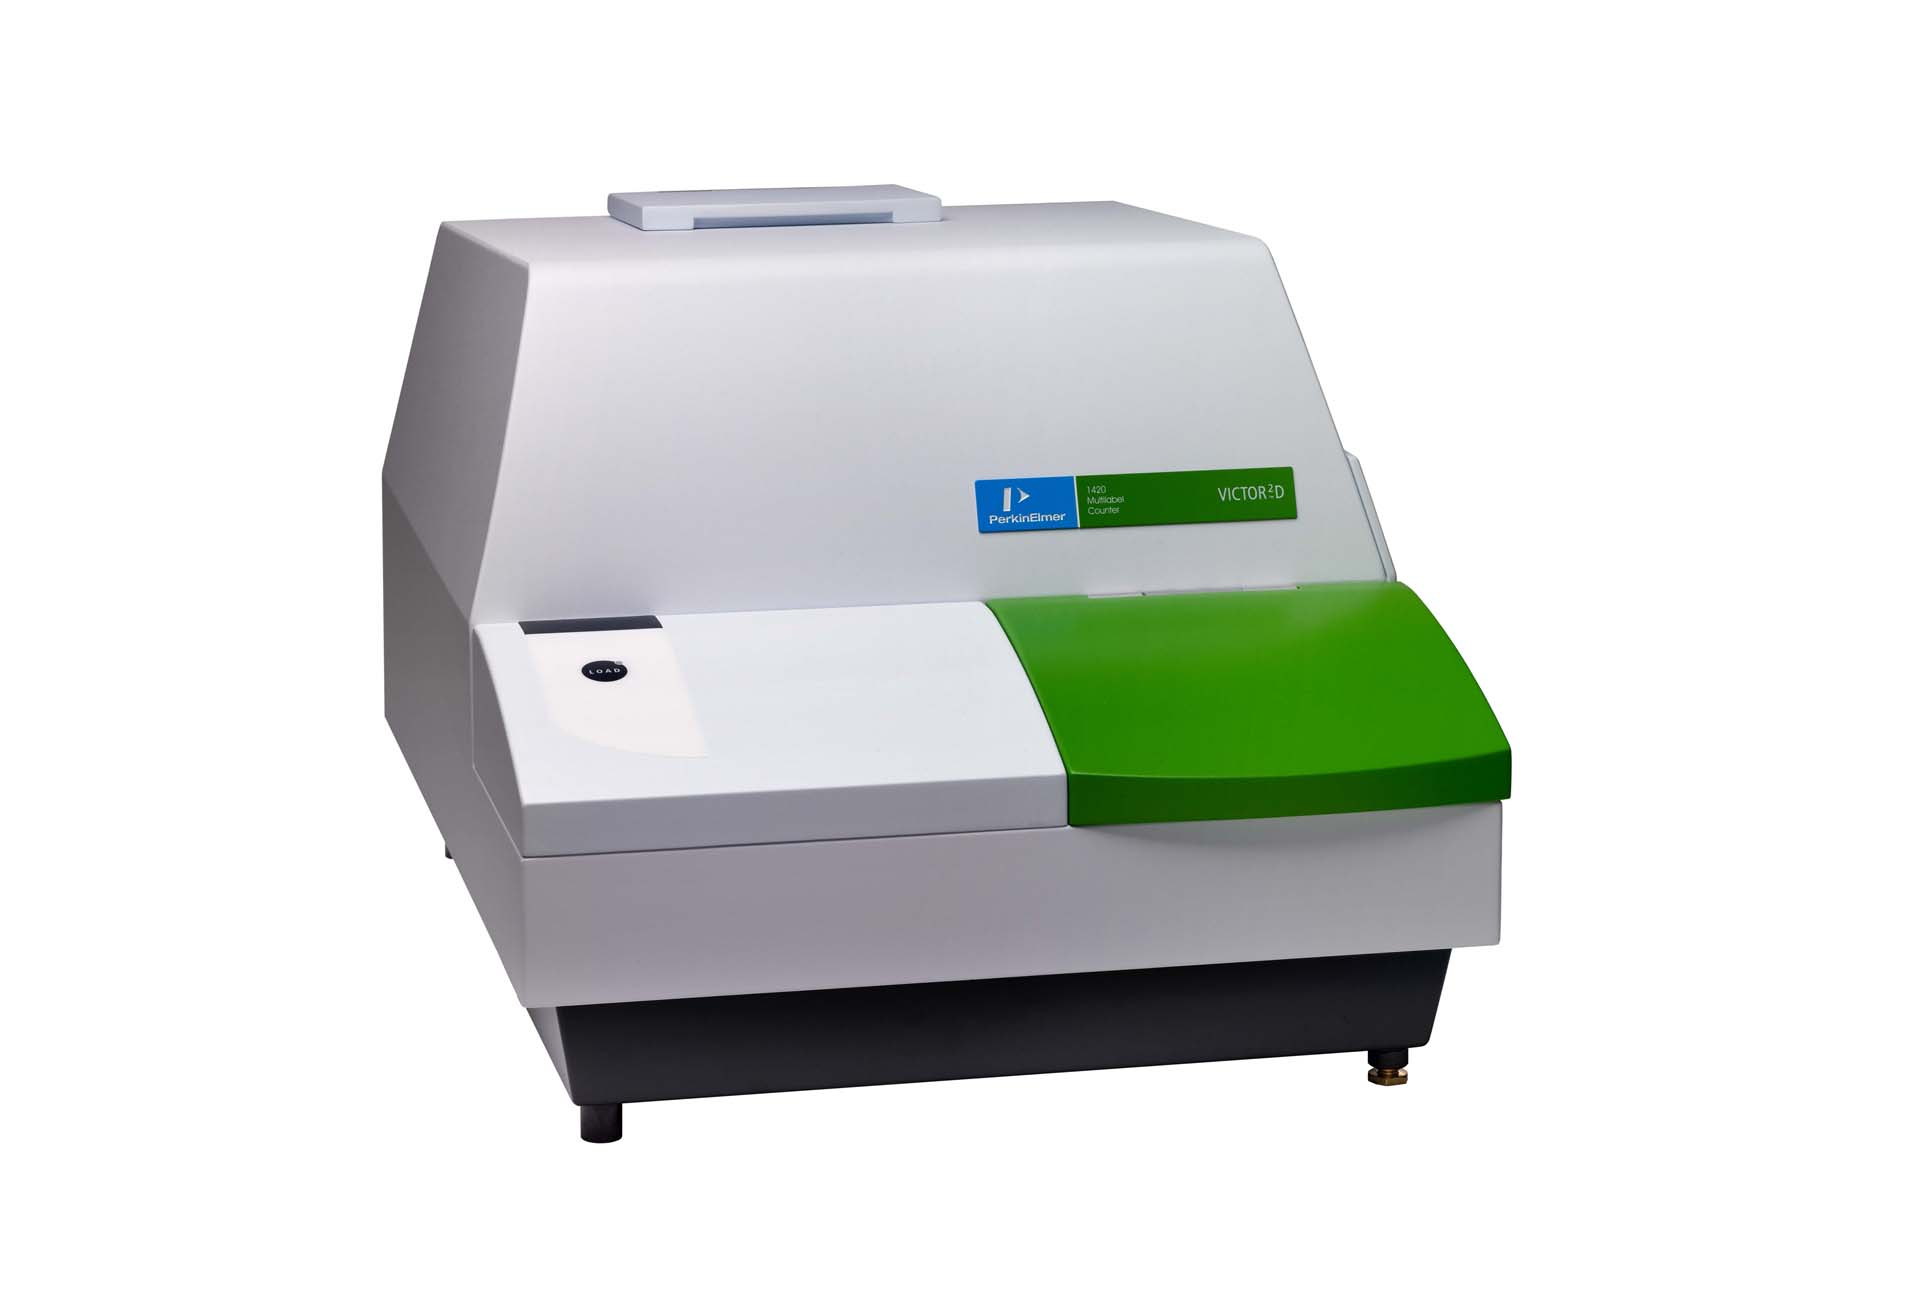
\includegraphics[width=5.5cm]{ch1/Victor-2D-72ppi}
    }
    \quad
    \subfigure[DELFIA® Xpress免疫分析仪平台]{
    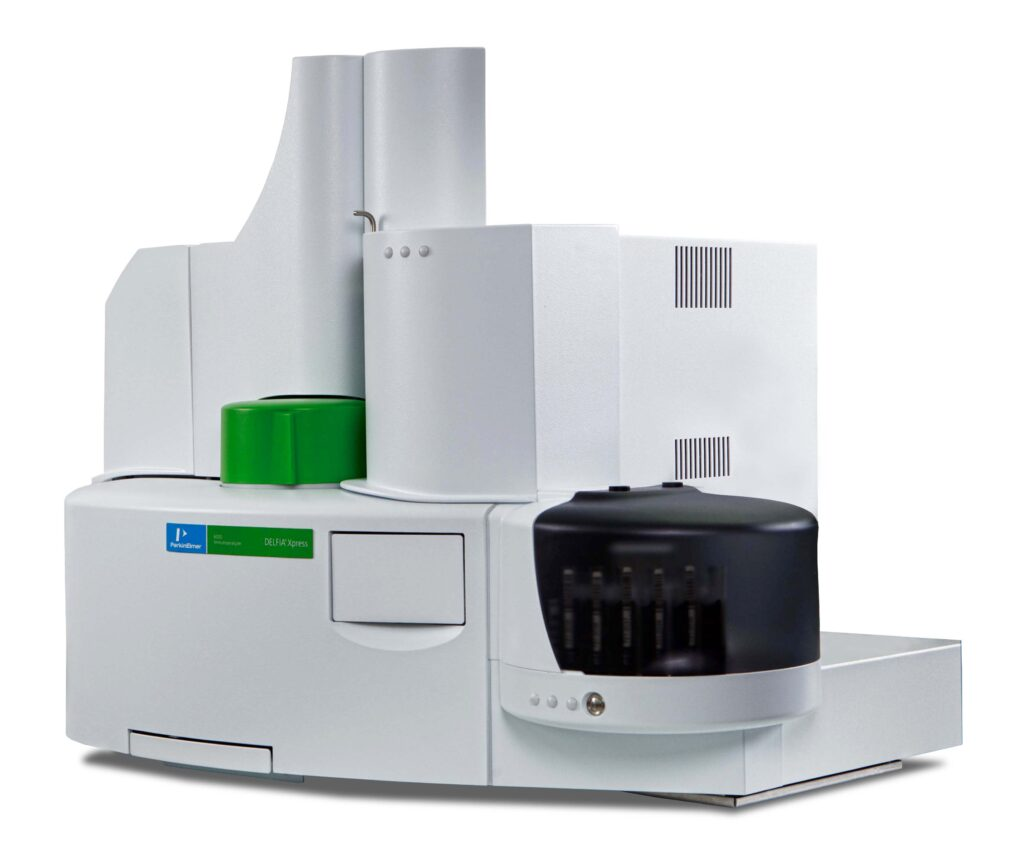
\includegraphics[width=5.5cm]{ch1/dx}
    }
    \caption{\label{fig:PerkinElmer}珀金埃尔默公司的两款检测设备}
\end{figure}

3. 中国宁波奥丞生物科技有限公司的荧光检测设备

作为中国新兴的医疗器械设备公司,奥丞专注于从疾病早期发现、诊断、预防到监测,力求通过提供可靠、快速与便捷的体外诊断产品为诊疗提供精准的检测结果。
目前,奥丞公司的多款化学荧光免疫平台产品均支持对PE生物标记物PLGF、sFlt-1等两种指标的检测\cite{aucheer2021}。此外,奥丞还根据实际临床需求,
提供了微小型床边诊断设备与大型实验室标定两种类型的设备,如\autoref{fig:aucheer}所示。
\begin{figure}[h]
    \centering
    \subfigure[微流控荧光免疫定量检测系统 iSort300]{
    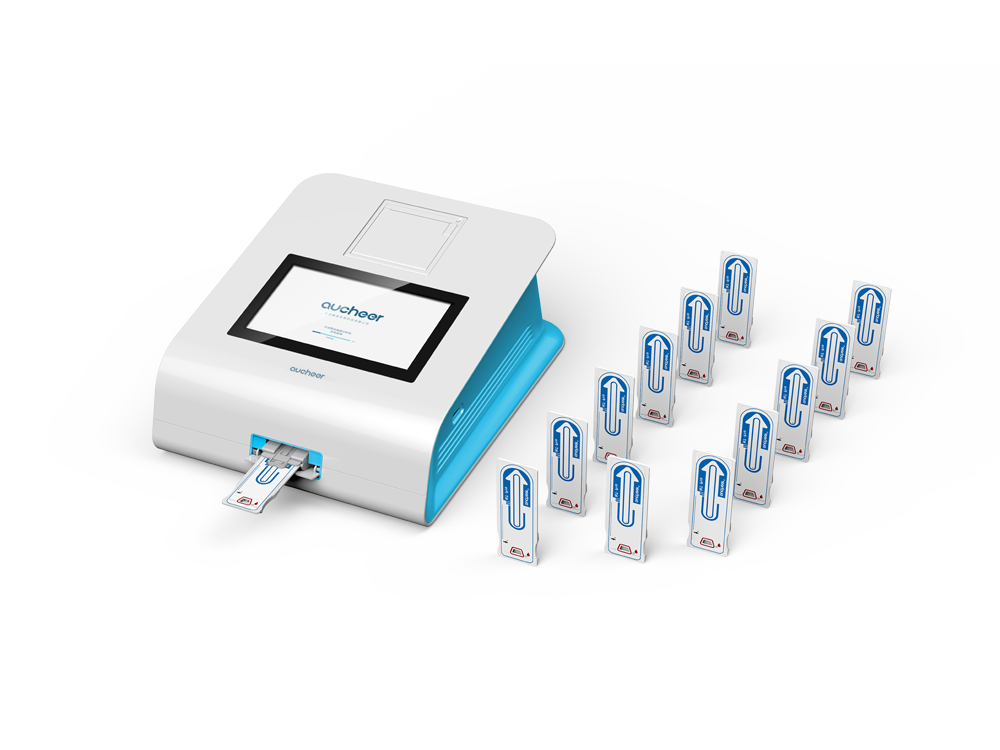
\includegraphics[width=5.5cm]{ch1/isort300}
    }
    \quad
    \subfigure[全自动化学发光免疫检测系统 Shine i1910]{
    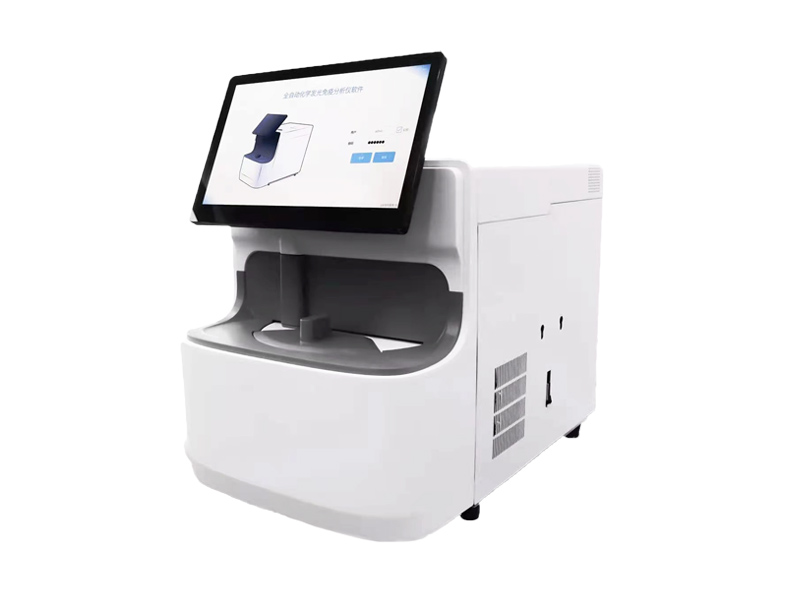
\includegraphics[width=5.5cm]{ch1/shinei1910}
    }
    \caption{\label{fig:aucheer}奥丞生物科技公司的荧光免疫平台}
\end{figure}


二、微型智能设备

随着移动智能医疗和可穿戴式设备的发展,通过微型智能设备实现对PE相关指标的实时、动态、多场景检测也逐渐成为了新的研究热点。但整体而言,基于智能设备的PE检测设备仍处于研发阶段,能真正实现多场景检测的成熟的PE分析系统尚未出现。
% 
% 2017年,Macarena Espinilla等人\cite{Espinilla2017}

2019年,Iuliana Marin等人\cite{Marin2019,Marin2020}通过一款智能腕部血压检测穿戴设备对孕妇的血压数据进行了监测,同时综合考虑孕妇的年龄、体重等风险因素,通过维特比动态规划算法(Viterbi algorithm),判断决策孕妇子痫前期
的患病可能,该系统原理框架图如\autoref{fig:mobile}所示。Iuliana Marin团队
通过对105名试验人员进行了测试,结果显示,最终的生成模型可以达到总体准确率80\%,敏感性为92.5\%,特异性为72\%\cite{Marin2019}。
\begin{figure}[htbp]
    \centering
    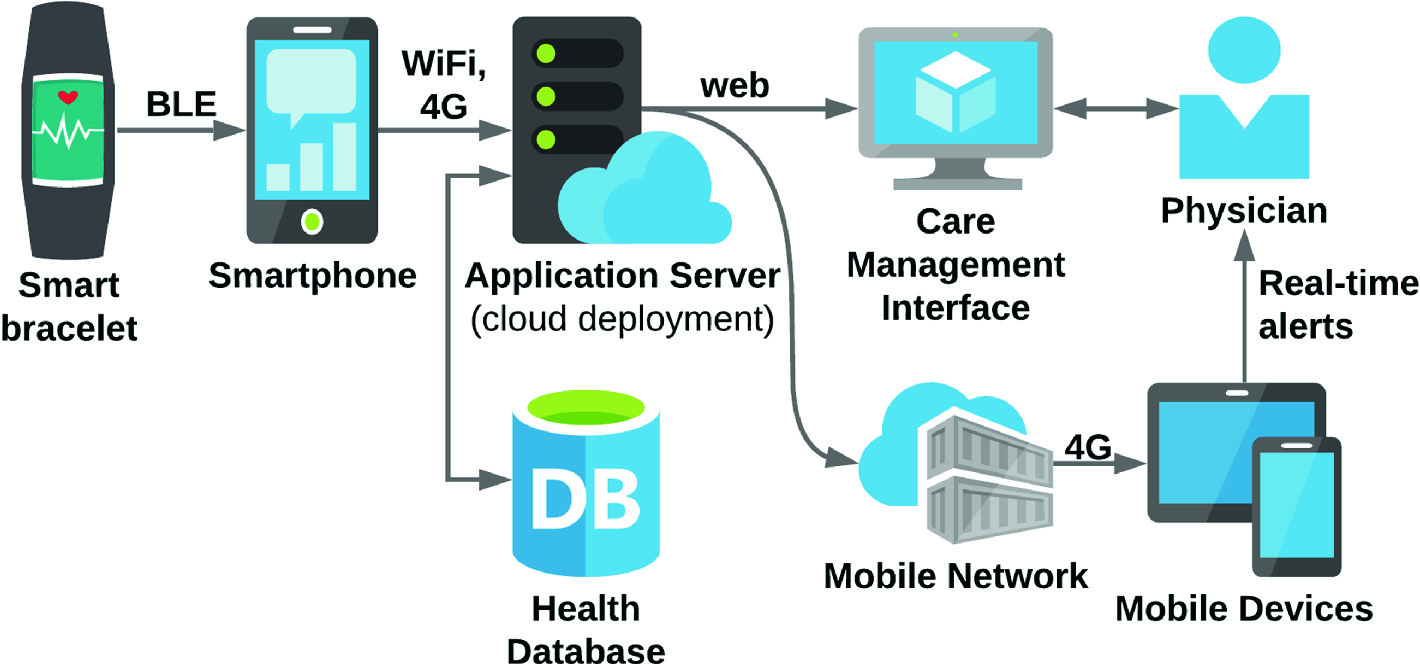
\includegraphics[width=.6\linewidth]{ch1/mobile}
    \caption{\label{fig:mobile}基于智能穿戴设备的血压检测系统框架图}
\end{figure}

\subsection{分析技术}
近年来,由于现代化设备的普遍使用致使医学检查过程各项数据激增,同时计算机领域人工智能技术的不断创新发展,相关研究者也开始尝试在子痫前期的识别、判断乃至预测等研究内容上引入人工智能技术。
利用人工智能技术分析前小节提到的各项风险因子、生理化学等参数一时间成为了炽手可热的多学科交叉研究点。
2016年,Rutvij Mehtad等\cite{Mehta2016}将大数据挖掘技术(Major Data Mining)在预测子痫前期、产科风险因素及产科其他疾病等健康领域的主要研究进行了归纳总结。他们将诸多学者的研究涉及的
数据挖掘与分析总结为两大类应用研究方向,即关联规则(Association Rule)挖掘方向与分类、聚类分析方向。关联规则挖掘力求发现多项数据之间的隐藏的逻辑与关系;分类分析是对通过现有数据建立模型预测新数据所属类别,
聚类分析则是按照一定规则将所有数据分组,使每组内的数据尽可能相似并有别于其他组数据\cite{Han2006}。在两大类应用的基础上,学者们使用不同的数据对子痫前期进行了分析研究。

一、数据挖掘

从众多的原始数据中筛选出与研究问题最为相关的部分,在实现数据降维的同时发现数据之间隐藏的联系是数据挖掘技术重要的研究内容。
如何从血浆代谢物、蛋白质及$mRNA$等生化指标中筛选出与PE患病最为相关的成份,此前的学者们也做了很多研究。

2005年,Louise C. Kenny等人\cite{Kenny2005}从利用基因遗传算法(genetic programming,GP),从血浆中代谢物成份确定特异的成份来识别患有PE的孕妇。他们通过对受试孕妇(其中,患有PE的实验组$N_{PE}=87$,正常对照组$N_{Normal}=87$,下同)
的血浆成份分析后,通过GP训练出了仅使用三种代谢物峰值变量预测模型。预测模型可以有效区分患有PE与正常孕妇,其灵敏度高达100\%,特异性高达98\%。

2020年,Jose F Carre˜no等人\cite{Carreno2020}基于蛋白质组学数据,改进了基于比较的特征选择算法进行了子痫前期的预测。特征算法包括帝国竞争与基因集簇两种降维算法与三点时间序列(分别对应孕前中晚期数据)总结算法两方面。
改进后的方法在两个独立数据集上均有90\%左右(85\%-93\%)的准确性,同时结果显示,孕早期与孕中期的蛋白质组学数据用以子痫前期的预测相较孕晚期结果会更准确。

2018年,Liron Yoffe等人\cite{Yoffe2018}对怀孕前三个月孕妇血浆中非编码循环RNA的丰度进行了分析,寻找能有效区分识别PE的转录RNA。他们在对孕妇的非编码RNA测序后,确定了实验组与对照组($N_{PE}=75$,$N_{Normal}=75$)
之间差异表达的25个RNA,最终训练生成了一个逻辑回归模型,经五层交叉验证,模型的AUC高达0.86。

同样是对RNA的研究,2021年Rong Guo等人\cite{Guo2021}则是利用集成学习投票决策算法筛选能够识别PE的胎盘mRNA。在获取了原始数据($N_{PE}=157$,$N_{Normal}=173$)后,他们基于相关性完成了数据降维,仅保留了原始48个差异表达基因中的13个。
同时通过构建了C4.5决策树(decision tree, DT)、自适应增强(adaptive boost, AdaBoost)及多层感知机(multilayer perceptron,MLP)三种分类器并通过多数投票策略,他们将分类识别准确性从开始的$79\%$提高至$82.2\%$。

2018年,Muhlis Tahir等人\cite{Tahir2018,Tahir2018-2}对比了利用神经网络和深度学习两种算法预测妊娠期孕妇PE的风险水平的结果。他们使用粒子群优化(PSO)作为特征选择算法,将原始数据集($N=1077$)的17个参数降维至9个。
在原始数据上通过LOO验证表明,深度学习后的模型具有95.12\%的准确率,使用经过缩减的数据集准确性还可提升至95.68\%。而当使用神经网络算法时,算法准确性亦可高达96.66\%。

二、 分类分析与聚类分析

所谓分类(Classification),就是按照某种标准给对象贴标签(label),再根据标签来区分归类;而聚类,则是在是指事先没有“标签”的情况下,通过某种聚集分析,找出事物之间存在聚集性原因的过程。分类分析与聚类分析是PE在机器学习领域最活跃的方向,而前文
提到的PE风险因子则是最为广泛使用的基础数据。

2017年,Pia M. Villa等人\cite{Villa2017}通过贝叶斯聚类算法,对受试孕妇(N=903)依据PE风险因子进行了聚类分析,对聚类结果分别计算了其PE患病可能。其聚类分析的热力度如\autoref{fig:Heatmap}所示。
结果PE的患病可能随孕妇具有的PE风险因子数量呈指数增长;同时,不同程度的PE往往其风险因子种类也有不同。
\begin{figure}[htbp]
    \centering
    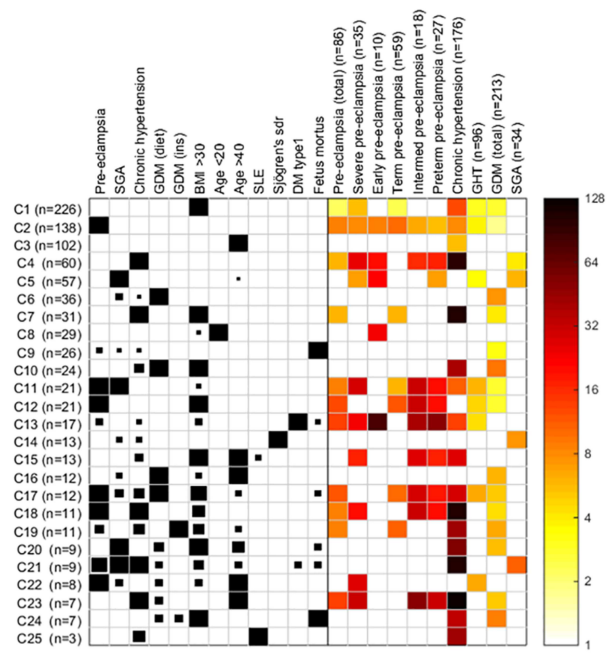
\includegraphics[width=.6\linewidth]{ch1/heatmap}
    \caption{\label{fig:Heatmap}热力图}
\end{figure}

2020年,Oknalita Simbolon等人\cite{Simbolon2020}基于软投票的集成学习算法,利用多项PE风险因子数据为PE患病高危孕妇开发了一款具有PE预测与推荐建议的智能手机APP。智能APP通过K近邻、线性支持向量机、RBF支持向量机、高斯过程、多层感知器和Ada-Boost等
6个单独的分类器分别对孕妇的PE患病可能进行预测,最后通过软投票的方法得出最佳预测模型并以此为孕妇给出相应的意见。通过对402例孕妇的数据测试表明,使用该算法最后能得到98.51\%±0.0186\%的高精度值,整体表现胜过其中任一单独分类器。

2011年,EDUARDO TEJERA等人\cite{Tejera2011}通过人工神经网络(Artificial neural network,ANN)完成了可对不同胎龄的正常孕妇、高血压孕妇及PE孕妇进行分类的模型构建。他们将\textbf{从ECG记录中获取的孕妇连续RR间期}($N=568$)与孕妇病史、血压值等其他风险因子结合作为模型输入。
最终训练所得的模型对PE识别的敏感性约为80\%,特异性约为85\%。

2020年,Ivana Mari{\'{c}}\cite{Maric2020}等人借助统计学习中的弹性网算法(Elastic Net Algorithm,ENA)从诸多可能导致子痫前期的风险因子等变量中训练了预测模型。经验证,该预测模型对子痫前期的预测ROC数值可以0.79,准确度可达45.2\%;模型对早发子痫前期预测的
ROC高达0.89,此时真阳性为72.3\%,假阳性为8.8\%。

2020年,Herdiantri Sufriyana等人\cite{Sufriyana2020-1}基于PE风险因子及生化指标(包括sFlt-1、UPTI与PlGF)对孕妇($N_{PE}=66$,$N_{Normal}=29$)PE发生情况进行了研究。经过特征筛选、多种模型性能对比,
他们最终通过M5P树状回归演算法训练获取的模型具有最佳分类效果,可实现100\%的精确度与95\%的敏感度。研究同时发现,最佳模型的特征是孕妇体重、BMI、UPTI、sFlt-1和PlGF,尤其是sFlt-1/PlGF比值。
同年,Sufriyana团队进行的另外一项研究\cite{Sufriyana2020}则聚焦于与PE相关的特征。他们对包含95个特征的印度尼西亚孕妇数据集($N_{PE}=3318$,$N_{Normal}=19883$)进行了建模分析。经筛选,最终由17项特征生成的随机森林模型对PE具有
最好的预测分析效果。

综上,基于机器学习的PE研究可总结为\autoref{tab:AIinPE}所示,由于篇幅内容所限,一些正文里未做介绍的研究也在\autoref{tab:AIinPE}中进行了补充。

\begin{center}
    \fontsize{10}{4}
    % Plan A
    % \setlength\LTleft{0pt}
    % \setlength\LTright{0pt}
	% \begin{longtable}{@{\extracolsep{\fill}}cccccc}
    % Plan B
    % 列宽总计16cm,各列按需分配长度,p{x-0.43cm}<{\centering}即可

    % \begin{longtable}{p{3cm}<{\centering}p{0.8cm}<{\centering}p{1.8cm}<{\centering}p{3.5cm}<{\centering}p{3cm}<{\centering}p{2cm}<{\centering}}
    \begin{longtable}{p{3cm}<{\centering}p{0.8cm}<{\centering}p{1.8cm}<{\centering}p{3.5cm}<{\centering}p{3cm}<{\centering}p{2cm}<{\centering}}
		\caption{基于机器学习的PE研究小结}\\
		\label{tab:AIinPE}\\
		\hline
            \textbf{研究者}&\textbf{时间}&\textbf{主要任务}&\tabincell{c}{\textbf{涉及的机器}\\\textbf{学习方法}}&\textbf{涉及参数}&\textbf{数据集规模}\\
        \hline
        \endfirsthead
        \caption[]{(续)}\\
        \hline
            \textbf{研究者}&\textbf{时间}&\textbf{主要任务}&\tabincell{c}{\textbf{涉及的机器}\\\textbf{学习方法}}&\textbf{涉及参数}&\textbf{数据集规模}\\
        \hline
        \endhead 
        \hline
        \endfoot
            Louise C. Kenny\cite{Kenny2005}&2005&降维、分类&基因遗传算法&多种血浆代谢物&\tabincell{c}{$N_{PE}=87,$\\$N_{Normal}=87$}\\
            Jose F Carre˜no\cite{Carreno2020}&2020&降维、分类&帝国竞争算法、基因集簇算法&\tabincell{c}{多种蛋白质\\组学物质}&$N=202$\\
            Liron Yoffe\cite{Yoffe2018}&2018&降维、分类&逻辑回归&非编码循环RNA&\tabincell{c}{$N_{PE}=75,$\\$N_{Normal}=75$}\\
            Rong Guo\cite{Guo2021}&2021&降维、分类&\tabincell{c}{集成学习、 C4.5决策树、\\自适应增强、多层感知机}&胎盘mRNA&\tabincell{c}{$N_{PE}=157,$\\$N_{Normal}=173$}\\
            Muhlis Tahir\cite{Tahir2018,Tahir2018-2}&2018&降维、分类&粒子群优化算法&PE风险因子&$N=1077$\\
            Pia M. Villa\cite{Villa2017}&2017&聚类分析&贝叶斯聚类算法&PE风险因子&$N=903$\\
            Oknalita Simbolon\cite{Simbolon2020}&2020&分类&集成学习软投票&PE风险因子&$N=402$\\
            EDUARDO TEJERA\cite{Tejera2011}&2011&分类&人工神经网络&\textbf{心电RR间期}及PE风险因子&$N=568$\\
            Ivana Mari{\'{c}}\cite{Maric2020}&2020&分类&弹性网算法&PE风险因子&$N=16370$\\
            % \multirow{2}{*}{Herdiantri Sufriyana\cite{Sufriyana2020-1,Sufriyana2020}}
            % &分类&M5P树状回归演算法&PE风险因子及生化指标&\tabincell{c}{$N_{PE}=66,$\\$N_{Normal}=29$}\\
            Herdiantri Sufriyana\cite{Sufriyana2020-1}&2020&分类&M5P树状回归演算法&PE风险因子及生化指标&\tabincell{c}{$N_{PE}=66,$\\$N_{Normal}=29$}\\
            Herdiantri Sufriyana\cite{Sufriyana2020}&2020&降维、分类&随机森林算法&PE风险因子及多项其他指标&\tabincell{c}{$N_{PE}=3318,$\\$N_{Normal}=19883$}\\
            Costas K. Neocleous\cite{Neocleous2009}\footnote{正文未做详细介绍,详情请参阅原文。\label{ft:note}}&2009&降维、分类&神经网络&PE风险因子及生化指标&$N=6838$\\
            Jong Hyun Jhee\cite{Jhee2019}\textsuperscript{\ref{ft:note}}&2009&模式识别、聚类分析&\tabincell{c}{逻辑回归、决策树、\\朴素贝叶斯、随机森林等}&PE风险因子及多项其他指标&$N=11006$\\
            Antonieta Martínez-Velasco\cite{Martinez2018}\textsuperscript{\ref{ft:note}}&2008&分类&多种机器学习算法&PE风险因子及多项其他指标&\tabincell{c}{$N_{PE}=269,$\\$N_{Normal}=1365$}\\
            Mário W. L. Moreira\cite{Moreira2016}\textsuperscript{\ref{ft:note}}&2016&降维、分类&贝叶斯网络&PE风险因子及多项生理症状&$N=164$\\
	\end{longtable}
\end{center}

\subsection{存在的不足与分析}
综合上述分析,对子痫前期的早期识别与检测可从按以下思路开展深入探索与研究。

但上述方法仍存在着一定的缺陷与不足:风险因素量表方法对具备多项子痫前期的风险因子的孕妇进行了一定的排除,但整体而言准确性不足,且无法反映孕期过程中的任何动态变化;而现有的
生理参数指标检测均需借助专业设备完成,有操作复杂、检测成本高、检测场地受限需有创采集等局限。此外,上述方法只能作为子痫前期的诊断之用,无法对整个孕期内子痫前期进行动态检测。因此,如何实现对子痫前期的便捷、快速、
无创、准确的临床诊断乃至全孕期内的监测仍有待进一步深入研究


\section{脉搏波在子痫前期领域研究现状}

而从无创检测的角度,光电容积脉搏波可以反应血液动力学的变化。因为脉搏波是心脏周期性搏动的体现,心脏的收缩和舒张引起的振动沿动脉血管和血流向外周传播从而
形成了脉搏波。由于血管直径富于变化,脉搏波到达之处血液流动速率也将发生一定的脉动变化,容积脉搏波包含了有关人体血液微循环方面的更富细节的生理信息
[17]。因此子痫前期导致的人体血液动力学改变,完全可以用光电容积脉搏波的特征来表示。同时光电容积脉搏波(Photoplethysmography, PPG)采集可无
创进行,具有采集过程定位简单、易于操作,信号质量高、稳定性强等特点,所以完全满足临床便捷、快速、无创的检测要求。

近年来,基于光电容积脉搏波的子痫前期的研究也有了进一步的发展。
\subsection{传统指标}
2018年,Tammy Y. Euliano等人\cite{Euliano2018}通过无创监测心电图与光电脉搏图对识别PE患者($N_{PE}=25$,$N_{Normal}=31$)进行了研究。他们发现PE患者的脉搏波波峰时长较正常孕妇长、弹性系数较正常孕妇小。
将这些脉搏波特征与其他心电特征训练得到的分类器的ROC数值高达0.907,敏感性78.2\%,特异性89.9\%。

2008年,KARLIJN VOLLEBREGT等人\cite{KARLIJN2008}研究了使用脉搏波数据进行PE初筛的可能。通过对健康孕妇($N=223$)的跟踪研究表明舒张压、心输出量与脉搏波增强指数均对PE预测模型有明显影响。结合PE风险因子,最终得到的模型
ROC数值可达0.95,其中敏感性90\%、特异性86\%。

2012年,Kathleen Tomsin等人\cite{Tomsin2012}对静脉脉搏波传播速度(Pulse Wave Velocity,PWV)进行了研究。研究结果显示在正常妊娠期孕妇所有脏器的PWV均呈现逐渐升高的趋势。
但子痫前期的早期(n=12)及晚期患者(n=14)的PWV数值较正常孕妇(n=16)数值更低。Ira Bernstein等人\cite{Ira2014}、MIHAELA VIVIANA IVAN等人\cite{VivianaIvan2018}及Irene Katsipi等人\cite{Katsipi2014}
的多项研究也进一步验证PWV在PE检测识别中的作用。

2014年,Su Fangming等人\cite{Su2014}的研究发现,可以通过光电容积脉搏波无创评估整个妊娠过程中心血管活动情况。他们提取分析了脉搏波增强指数(AIX)、反射指数(RI)、传导时间(PTT)等,
发现这些参数随者妊娠时间的增长在孕期内均有统计意义上的明显改变。

2014年,Nan Han等人\cite{Han2014}研究孕妇心血管系统与子宫动脉血流系统的一致性也得到了与Kathleen Tomsin等人\cite{Tomsin2012}类似的结论。他们以三个月为单位对子宫动脉多普勒超声与指端光电容积脉搏波的检测结
果进行了对比分析($N_{PE}=10$,$N_{Normal}=80$)。结果显示,正常孕妇的子宫动脉阻力指数(UtA RI)与脉搏波反射指数(RI)均随妊娠时间的延长而显著降低,且趋势基本一致。而PE患者的两项参数的数值均明显高于正常孕妇。

\subsection{新型指标}
2018年,Ying Feng等人\cite{Feng2018}基于光电容积脉搏波提出了差异面积比参数(ADR),发现子痫前期会导致孕妇ADR较正常妊娠孕妇低;

2019年,陈婉琳等人\cite{Chen2019}基于光电容积脉搏波提出了光电容积斜率指数(photoplethysmography slope index,PSI),并通过对50例孕妇(子痫患者23例,正常孕妇27例)的脉搏波数据对PSI进行了检验,
结果表明其灵敏性和特异性分别达到 87.0\%和 96.3\%,准确性达到 92.0\%。

上述研究证明,\textbf{子痫前期患者的血流动力学变化与光电容积脉搏波之间确实存在着一定的联系},但更进一步的研究亟待开展
容积脉搏波蕴含着丰富的关于人体血液微循环的信息,除动脉血流量、脉搏波速度指数等参数之外,\textbf{更多特征参数有待挖掘}。
综上,基于机器学习的PE研究可总结为\autoref{tab:PPGinPE}所示。

\begin{center}
    \fontsize{10}{4}
	\begin{longtable}{p{3cm}<{\centering}p{1cm}<{\centering}p{2cm}<{\centering}p{6cm}<{\centering}p{1cm}<{\centering}}
		\caption{基于脉搏波的PE研究小结}\\
		\label{tab:PPGinPE}\\
		\hline
            \textbf{研究者}&\textbf{时间}&\textbf{脉搏波参数}&\textbf{研究结果}&\textbf{备注}\\
        \hline
        \endfirsthead
        \caption[]{(续)}\\
        \hline
            \textbf{研究者}&\textbf{时间}&\textbf{脉搏波参数}&\textbf{研究结果}&\textbf{备注}\\
        \hline
        \endhead 
        \hline
        \endfoot
	\end{longtable}
\end{center}

\section{研究目标与研究内容}

\subsection{研究目标}
综合应用各种方法,提取研发新型光电容积脉搏波形态学特征参数,构建一般通用的光电容积脉搏波的描述特征集合。在此基础上,通过特征筛选、压缩等算法提取出对子痫前期有一定甄别能力的特征集,
使用机器学习算法构建出子痫前期筛选识别模型,并对最终模型的性能表现进行验证评估。
\subsection{研究内容}
全文研究内容可分为数据源获取、信号预处理、特征参数提取与分析、子痫前期甄别模型训练构建及模型评估具体包括5个部分,如所示。每部分具体研究内容包括:
\begin{enumerate}
    \item 数据源获取。介绍本研究所采用的数据来源(临床现场采集),包括采集设备、采集流程及规范。  
    \item 信号预处理。对从硬件设备获取的PPG信号分析其信号成分特点,完成滤波去噪、去基线漂移、特征点检测及标准化等准备工作。
    \item 特征参数提取与分析。从脉搏波形态学等方面构建特征参数。
    \item 子痫前期甄别模型训练构建及评估。通过机器学习中的等方法构建子痫前期甄别模型,并验证模型准确性。
    \item 模型评估。
\end{enumerate}

\textbf{各章节的具体内容安排如下:}

第一章是绪论。介绍子痫前期的定义及危害,梳理了目前临床已应用的检测方法及指标,分析各项方法的缺陷与不足。最后确定提出了本文的研究目标与内容。

第二章是光电容积脉搏波概述。阐述了

第三章是光电容积脉搏波的特征点检测算法。

第四章是光电容积脉搏波的特征集构建。

第五章是基于光电容积脉搏波特征的子痫前期检测识别模型。通过等几种方法优化特征参数集并构建了子痫前期的甄别模型,通过等方面评估了各项模型的整体性能表现。

第六章是低耦合高拓展的软件综合分析系统的设计与实现。阐述了本研究包括数据源导入管理、预处理算法管理、特征拓展管理、标准数据管理、模型训练生成管理等方面在内的整体分析系统的软件设计思路,
介绍了为提高本研究各部分内的内聚性、降低各研究内容之间的耦合性、提高系统整体可拓展性及实用性、提高系统真正落地临床的可能性所做出的各项规划及实现。

第七章是总结与展望。对本论文的全部研究工作进行系统性总结,阐述本论文的创新工作点,并对下一阶段的研究工作内容进行了规划与展望。